\documentclass{article}
\usepackage{amsmath}
\usepackage{amsmath, amssymb, amsthm}
\usepackage{tikz}

\begin{document}

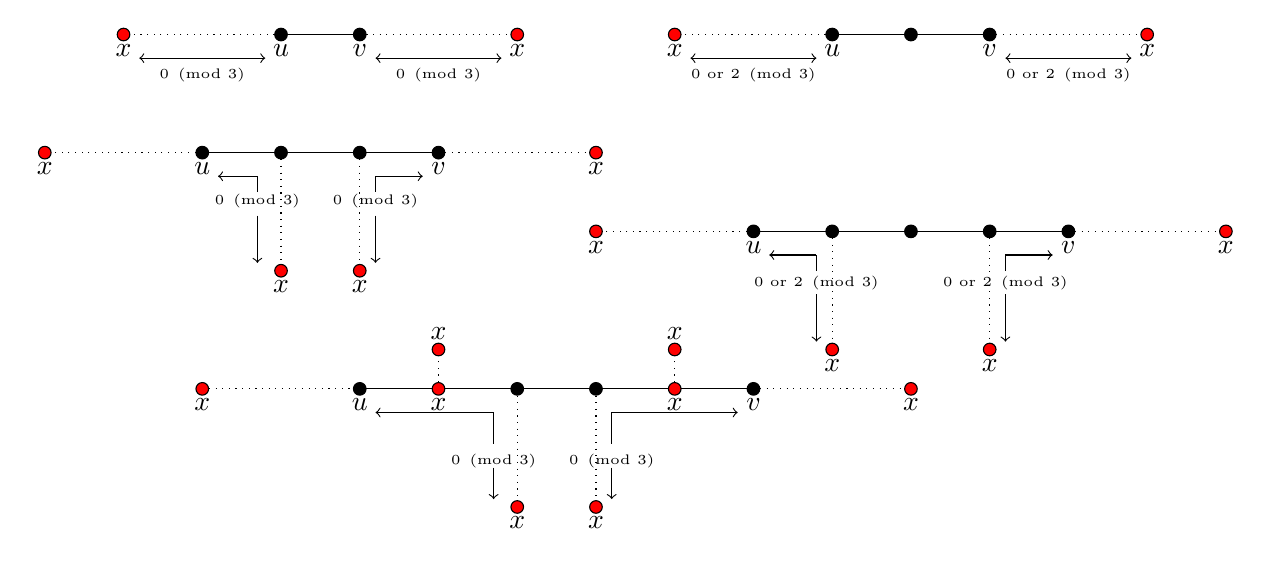
\begin{tikzpicture}

\draw[dotted] (-8,0)--(-10,0); \draw (-8,0)--(-7,0);\draw[dotted] (-7,0)--(-5,0);
\draw[<->] (-9.8,-.3)--(-8.2,-.3); \draw[<->] (-6.8,-.3)--(-5.2,-.3);

\draw  [fill=black](-8,0) circle [radius=0.08]; \draw  [fill=red](-10,0) circle [radius=0.08]; \draw  [fill=black](-7,0) circle [radius=0.08]; \draw  [fill=red](-5,0) circle [radius=0.08]; 

\node [below] at (-8,0) {$u$}; \node [below] at (-7,0) {$v$}; \node [below] at (-5,0) {$x$}; \node [below] at (-10,0) {$x$};

\node [below, font=\tiny] at (-9,-.3) {$0 \pmod 3$}; \node [below, font=\tiny] at (-6,-.3) {$0 \pmod 3$};


%%%%%% Second Figure 
\draw[dotted] (-1,0)--(-3,0); \draw (-1,0)--(1,0); \draw[dotted] (1,0)--(3,0); 
\draw[<->] (-2.8,-.3)--(-1.2,-.3); \draw[<->] (1.2,-.3)--(2.8,-.3);

\draw  [fill=black](-1,0) circle [radius=0.08]; \draw  [fill=black](0,0) circle [radius=0.08]; \draw  [fill=black](1,0) circle [radius=0.08]; \draw  [fill=red](-3,0) circle [radius=0.08]; \draw  [fill=red](3,0) circle [radius=0.08];

\node [below] at (-1,0) {$u$}; \node [below] at (1,0) {$v$}; \node [below] at (3,0) {$x$}; \node [below] at (-3,0) {$x$};

\node [below, font=\tiny] at (-2,-.3) {$0$ or $2 \pmod 3$}; \node [below, font=\tiny] at (2,-.3) {$0$ or $2 \pmod 3$};


%%%%% Third Figure 
\draw[dotted] (-9,-1.5)--(-11,-1.5); \draw (-9,-1.5)--(-6,-1.5);\draw[dotted] (-6,-1.5)--(-4,-1.5); \draw[dotted] (-8,-1.5)--(-8,-3);\draw[dotted] (-7,-1.5)--(-7,-3);

\draw[<-] (-8.8,-1.8)--(-8.3,-1.8); \draw (-8.3,-2)--(-8.3, -1.8);\draw[->] (-8.3,-2.3)--(-8.3,-2.9);
\draw[->] (-6.8,-1.8)--(-6.2,-1.8);\draw (-6.8,-1.8)--(-6.8,-2);\draw[->] (-6.8,-2.3)--(-6.8,-2.9);

\draw  [fill=black](-9,-1.5) circle [radius=0.08]; \draw  [fill=black](-8,-1.5) circle [radius=0.08];\draw  [fill=black](-7,-1.5) circle [radius=0.08];
\draw  [fill=black](-6,-1.5) circle [radius=0.08];\draw  [fill=red](-11,-1.5) circle [radius=0.08];\draw  [fill=red](-4,-1.5) circle [radius=0.08];
\draw  [fill=red](-8,-3) circle [radius=0.08];\draw  [fill=red](-7,-3) circle [radius=0.08];


\node [below] at (-9,-1.5) {$u$}; \node [below] at (-6,-1.5) {$v$};\node [below] at (-11,-1.5) {$x$};\node [below] at (-4,-1.5) {$x$}; \node [below] at (-8,-3) {$x$}; \node [below] at (-7,-3) {$x$}; 

\node [below, font=\tiny] at (-8.3,-1.9) {$0 \pmod 3$}; \node [below, font=\tiny] at (-6.8,-1.9) {$0 \pmod 3$};


%%%%% Fourth figure
\draw[dotted] (-2,-2.5)--(-4,-2.5); \draw (-2,-2.5)--(2,-2.5); \draw[dotted] (2,-2.5)--(4,-2.5);\draw[dotted] (-1,-2.5)--(-1,-4);\draw[dotted] (1,-2.5)--(1,-4);

\draw[<-] (-1.8,-2.8)--(-1.2,-2.8); \draw (-1.2,-2.8)--(-1.2, -3);\draw[->] (-1.2,-3.3)--(-1.2,-3.9);
\draw[->] (1.2,-2.8)--(1.8,-2.8);\draw (1.2,-2.8)--(1.2,-3);\draw[->] (1.2,-3.3)--(1.2,-3.9);

\draw  [fill=black](-2,-2.5) circle [radius=0.08]; \draw  [fill=black](-1,-2.5) circle [radius=0.08]; \draw  [fill=black](0,-2.5) circle [radius=0.08]; \draw  [fill=black](1,-2.5) circle [radius=0.08]; \draw  [fill=black](2,-2.5) circle [radius=0.08];
\draw  [fill=red](-4,-2.5) circle [radius=0.08]; \draw  [fill=red](4,-2.5) circle [radius=0.08];\draw  [fill=red](-1,-4) circle [radius=0.08];\draw  [fill=red](1,-4) circle [radius=0.08];

\node [below] at (-2,-2.5) {$u$}; \node [below] at (2,-2.5) {$v$}; \node [below] at (-4,-2.5) {$x$}; \node [below] at (4,-2.5) {$x$};

\node [below] at (-1,-4) {$x$}; \node [below] at (1,-4) {$x$};

\node [below, font=\tiny] at (-1.2,-2.95) {$0$ or $2 \pmod 3$}; \node [below, font=\tiny] at (1.2,-2.95) {$0$ or $2 \pmod 3$};



%%%%%%%% Fifth figure

\draw[dotted] (-9,-4.5)--(-7,-4.5);\draw (-7,-4.5)--(-2,-4.5); \draw[dotted] (-2,-4.5)--(0,-4.5); \draw[dotted] (-5,-4.5)--(-5,-6); \draw[dotted] (-4,-4.5)--(-4,-6);

\draw[<-] (-6.8,-4.8)--(-5.3,-4.8);\draw (-5.3,-4.8)--(-5.3, -5.2);\draw[->] (-5.3,-5.5)--(-5.3,-5.9);

\draw[->] (-3.8,-4.8)--(-2.2,-4.8); \draw (-3.8,-4.8)--(-3.8,-5.2); \draw[->] (-3.8,-5.5)--(-3.8,-5.9);

\draw[dotted] (-6,-4.5)--(-6,-4);
\draw[dotted] (-3,-4.5)--(-3,-4);

\draw [fill=red](-6,-4) circle [radius=0.08]; 
\draw [fill=red](-3,-4) circle [radius=0.08];

\draw  [fill=black](-7,-4.5) circle [radius=0.08];\draw  [fill=red](-6,-4.5) circle [radius=0.08];\draw  [fill=black](-5,-4.5) circle [radius=0.08];
\draw  [fill=black](-4,-4.5) circle [radius=0.08]; \draw  [fill=red](-3,-4.5) circle [radius=0.08]; \draw  [fill=black](-2,-4.5) circle [radius=0.08];
\draw  [fill=red](0,-4.5) circle [radius=0.08]; \draw  [fill=red](-9,-4.5) circle [radius=0.08]; \draw  [fill=red](-5,-6) circle [radius=0.08];
\draw  [fill=red](-4,-6) circle [radius=0.08];


\node [below] at (-7,-4.5) {$u$}; \node [below] at (-2,-4.5) {$v$}; \node [below] at (-9,-4.5) {$x$}; \node [below] at (0,-4.5) {$x$}; \node [below] at (-5,-6) {$x$}; \node [below] at (-4,-6) {$x$};
\node [below] at (-6,-4.5){$x$};
\node [below] at (-3,-4.5){$x$};
\node[above] at (-6,-4){$x$};
\node[above] at (-3,-4){$x$};

\node [below, font=\tiny] at (-3.8,-5.2) {$0 \pmod 3$}; \node [below, font=\tiny] at (-5.3,-5.2) {$0 \pmod 3$};

\end{tikzpicture}

\end{document}